% =====================================================================
%  TELFOR 2026 -- Telekomunikacioni forum, Beograd
%  Rad: O konfiguracijama pohrane za HTAP u SQL Serveru 2022:
%       empirijska evaluacija
%  Autori: Nejra Smajlović (Univerzitet u Zenici, Politehnički fakultet)
%          Alen Begović (Univerzitet u Sarajevu, Elektrotehnički fakultet)
%
%  BOSANSKA VERZIJA rada telfor2026_htap.tex. Sadržaj, brojke i zaključci
%  su identični; razlikuje se samo jezik i decimalni zarez.
%
%  USKLAĐENOST S TELFOR PRAVILIMA:
%    * dvokolonski A4, standardni IEEE konferencijski template (IEEEtran, 10 pt)
%    * najviše 4 stranice A4 za redovne i studentske radove
%
%  Build:  pdflatex telfor2026_htap_bs.tex   (pokrenuti dva puta)
% =====================================================================
\documentclass[10pt,conference,a4paper]{IEEEtran}
\IEEEoverridecommandlockouts

\usepackage[T1]{fontenc}
\usepackage[utf8]{inputenc}
\usepackage[croatian]{babel}   % prelamanje riječi; bosanski nema zaseban obrazac
\usepackage{cite}
\usepackage{graphicx}
\usepackage{amsmath}
\usepackage{booktabs}
\usepackage{balance}
\usepackage{url}
\usepackage[hidelinks]{hyperref}

% --- Nazivi elemenata na bosanskom -----------------------------------
\renewcommand{\abstractname}{Sažetak}
\renewcommand{\IEEEkeywordsname}{Ključne riječi}
\renewcommand{\refname}{Literatura}
\renewcommand{\figurename}{Slika}
\renewcommand{\tablename}{Tabela}

% --- Tipografija tabela ----------------------------------------------
\newcommand{\best}[1]{\textbf{#1}}

% --- Copyright napomena na dnu prve stranice -------------------------
% TELFOR u uputstvu za autore ne trazi IEEE copyright liniju na radu koji se
% predaje, a nema je ni zvanicni IEEE konferencijski template, pa se rad
% predaje bez nje umjesto s rezerviranim mjestom. Ako TELFOR objavi copyright
% string za finalnu verziju, otkomentarisati tri linije ispod i upisati ga.
%\IEEEpubid{\parbox{\columnwidth}{\footnotesize
%  978-1-XXXX-XXXX-X/26/\$31.00~\copyright2026 IEEE\hfill}
%  \hspace{\columnsep}\makebox[\columnwidth]{}}

\begin{document}

\title{O konfiguracijama pohrane za HTAP u SQL\\
Serveru 2022: empirijska evaluacija}

\author{\IEEEauthorblockN{Nejra Smajlović}
\IEEEauthorblockA{\textit{Univerzitet u Zenici}\\
\textit{Politehnički fakultet}\\
Zenica, Bosna i Hercegovina\\
nejra.smajlovic.22@size.ba}
\and
\IEEEauthorblockN{Alen Begović}
\IEEEauthorblockA{\textit{Univerzitet u Sarajevu}\\
\textit{Elektrotehnički fakultet}\\
Sarajevo, Bosna i Hercegovina\\
alen.begovic@etf.unsa.ba}%
\thanks{N. Smajlović je s Politehničkog fakulteta Univerziteta u Zenici, a
A. Begović s Elektrotehničkog fakulteta Univerziteta u Sarajevu, Bosna i
Hercegovina. Izvorni kod benchmarka, SQL skripte i mjerenja:
\url{https://github.com/itsnejra/htap-sqlserver-benchmark}.}}

\maketitle

\begin{abstract}
Ovaj rad donosi nezavisnu empirijsku evaluaciju četiri strategije pohrane
dostupne unutar jedne instance Microsoft SQL Servera 2022, namijenjenu
sistemima koji nad istim podacima moraju opsluživati transakcijske i
analitičke upite bez zastarjelosti i operativne složenosti koje uvodi
skladište premošćeno ETL procesom: disk-zasnovane tabele s B-stablo
indeksima (Baseline), disk-zasnovane tabele
s nonclustered columnstore indeksom (CS), memorijsko-optimizirane tabele na
Hekaton engineu (IM) i hibridnu dual-store konfiguraciju koja
memorijsko-optimizirani transakcijski sloj kombinuje s columnstore
analitičkim slojem (HTAP). Eksperiment je puni faktorijalni dizajn nad
četiri konfiguracije, tri omjera OLTP/OLAP i tri razine konkurentnosti, s 30
ponavljanja po ćeliji, nad skupom podataka StackOverflow2010 od približno
19,2 miliona zapisa po shemi; 1.070 valjanih serija analizirano je
Kruskal-Wallisovim H testom, Mann-Whitneyevim U testom s Bonferroni
korekcijom, Cohenovim d i log-linearnom OLS regresijom. Dual-store
konfiguracija dominira u svakom ispitanom scenariju: ostvaruje 3,3 do 6,9
puta veću OLTP propusnost od čisto memorijsko-optimizirane konfiguracije pri
transakcijski intenzivnom opterećenju i smanjuje medijanu analitičke
latencije za faktor četiri u odnosu na Baseline. Budući da razdvaja
dva sloja bez ikakve cijene sinhronizacije tokom mjerenja, prikazani dobici
predstavljaju gornju granicu pristupa.
\end{abstract}

\begin{IEEEkeywords}
HTAP, In-Memory OLTP, columnstore indeks, SQL Server 2022, benchmarking baza
podataka, izolacija performansi.
\end{IEEEkeywords}

% =====================================================================
\section{Uvod}
% =====================================================================
\IEEEPARstart{S}{avremeni} informacioni sistemi moraju opsluživati dvije
klase opterećenja sa suprotstavljenim zahtjevima. Transakcijska obrada
(OLTP) sastoji se od kratkih atomarnih operacija nad pojedinačnim zapisima
pri visokoj konkurentnosti i uz stroge zahtjeve konzistentnosti; analitička
obrada (OLAP) počiva na dugotrajnim upitima koji agregiraju milione zapisa i
traže visok propusni opseg čitanja. Tri decenije standardni odgovor na tu
napetost bila je arhitekturalna podjela: operativna baza premošćena prema
skladištu podataka ETL (extract-transform-load) procesom čije se kašnjenje
mjeri satima ili danima.
Hibridna transakcijsko-analitička obrada (HTAP), termin koji je Gartner uveo
2014. godine, označava klasu sistema koja teži eliminaciji tog
posrednika~\cite{ozcan2017}.

Microsoft SQL Server 2022 za tu svrhu nudi dva ugrađena mehanizma: Hekaton
in-memory OLTP engine~\cite{diaconu2013} i columnstore
indekse~\cite{larson2013}. Kako ih treba kombinovati pod mješovitim
opterećenjima nije sistematski ispitano izvan publikacija samog
proizvođača: dostupne benchmarking studije usmjerene su na distribuirane
NewSQL sisteme ili se oslanjaju na sintetičke skupove podataka (TPC-C,
TPC-H) čije uniformne distribucije pristupa ne reprodukuju Pareto raspodjelu
aktivnosti svojstvenu stvarnim web aplikacijama~\cite{zhang2024hybench}.

Ovaj rad adresira tu prazninu punim faktorijalnim benchmarkom četiri
konfiguracije pohrane unutar jedne instance SQL Servera 2022 nad stvarnim
skupom podataka. Doprinosi su: nezavisna, statistički rigorozna usporedba
četiri konfiguracije kroz tri omjera opterećenja i tri razine konkurentnosti
(1\,070 valjanih serija); kvantifikacija gubitka OLTP propusnosti koji svaka
konfiguracija trpi zbog istovremene analitike, s mehanizmom koji stoji iza
toga; te smjernice za odabir konfiguracije, uz preduslove pod kojima
vrijede.

% =====================================================================
\section{Dosadašnja istraživanja}
% =====================================================================
Zhang i drugi~\cite{zhang2024survey} klasifikuju HTAP sisteme prema
arhitekturi pohrane u četiri porodice, od primarne redne pohrane s in-memory
stupčastim indeksom do primarne stupčaste pohrane s rednim delta slojem.
Song i drugi~\cite{song2024} razdvajaju monolitne arhitekture, u kojima jedan
engine opslužuje oba radna toka, od hibridnih s razdvojenim engineima, i
zaključuju da je sposobnost održavanja stabilnih OLTP performansi pod
analitičkim opterećenjem smislenija mjera kvalitete od vršne propusnosti.

Komercijalni sistemi pokrivaju taj raspon. SAP HANA~\cite{farber2012} i
Oracle Database In-Memory~\cite{lahiri2015} drže redni i stupčasti format
unutar jednog in-memory enginea, dok TiDB~\cite{huang2020} razdvaja
transakcijski sloj (TiKV) od analitičkog (TiFlash) i sinhronizuje ih
asinhronom Raft replikacijom, postižući izolaciju po cijenu mrežne
latencije, a Google F1 Lightning~\cite{yang2020} pušta transakcijske
promjene u delta strukture koje kompakcija prepisuje u analitički format. SQL Server 2022 ostvaruje in-process varijantu istog obrasca i ne
plaća mrežnu latenciju. Njegovi gradivni elementi dobro su dokumentovani:
Hekaton engine~\cite{diaconu2013}, koji donosi ubrzanja od 10 do 30 puta za
točkaste upite, ali ne podržava ni indeksiranje pogodno za rasponska
skeniranja ni batch-mode izvršavanje, te columnstore
indeksi~\cite{larson2013}, čiji batch-mode executor obrađuje oko 1\,000
redova odjednom i daje ubrzanja od 10 do 100 puta na tipičnim skladišnim
upitima. Njihova kombinacija opisana je u~\cite{larson2015}, gdje su
prikazani dizajn i interni mikro-benchmarkovi autora samog sistema.

Metodološki, HyBench~\cite{zhang2024hybench} spaja TPC-C transakcije s
analitičkim upitima, Wu i drugi~\cite{wu2025} potvrđuju da dodatni
analitički klijenti izazivaju pad OLTP propusnosti koji se pojačava s
konkurentnošću, a Zhao i drugi~\cite{zhao2023} tvrde da izolacija
performansi treba biti primarni kriterij; noviji
sistemi~\cite{zhao2025pushtap, zhang2025synchro, zhan2025} pokazuju da
optimalna konfiguracija ovisi o interakciji profila opterećenja i
konkurentnosti, što motiviše primijenjeni faktorijalni dizajn.
Nezavisne evaluacije mehanizama SQL Servera ipak su rijetke, a nijedna
autorima poznata studija ne obuhvata tri razine konkurentnosti i tri omjera
uz neparametarsku analizu.

Istraživanje je organizovano oko tri pitanja. Prvo, kako se analitička
latencija disk-zasnovane columnstore konfiguracije odnosi prema hibridnoj i
mijenja li se to s konkurentnošću. Drugo, koliko transakcijske propusnosti
svaka konfiguracija ustupa kada analitički upiti rade uporedo s njom. Treće,
dobija li hibridna konfiguracija na propusnosti u odnosu na čisto
memorijsko-optimiziranu pri transakcijski intenzivnom opterećenju, s obzirom
da obje počivaju na istom Hekaton engineu.

% =====================================================================
\section{Posmatrani sistem}
% =====================================================================
Četiri konfiguracije implementirane su kao zasebne sheme (\texttt{baseline},
\texttt{cs}, \texttt{im}, \texttt{htap}) unutar jedne instance SQL Servera
2022, s identičnom logičkom strukturom tabela i identičnim podacima, ali
različitim fizičkim mehanizmima pohrane i indeksiranja. \emph{Baseline},
kontrolna grupa, koristi disk-zasnovane redne tabele s B-stablo indeksima i
row-mode izvršavanjem; \emph{CS} svakoj tabeli dodaje nonclustered
columnstore indeks, pa optimizator za analitičke upite bira batch-mode
planove dok OLTP naredbe i dalje koriste B-stablo. \emph{IM} koristi
memorijsko-optimiziranu pohranu (\texttt{MEMORY\_OPTIMIZED = ON},
\texttt{DURABILITY = SCHEMA\_ONLY}) s hash indeksima, rasponskim indeksima i
nativno kompajliranim OLTP procedurama, a analitičke upite nužno izvršava u
row-modu. \emph{HTAP} ostvaruje dual-store obrazac TiDB/TiFlash-a~\cite{huang2020}
u in-process modelu: pisanja i točkasta čitanja idu na
memorijsko-optimizirane tabele u shemi \texttt{htap}, dok analitički upiti
čitaju columnstore kopiju u shemi \texttt{cs}. Bile su potrebne dvije
postavke specifične za engine: \texttt{OPTION (MAXDOP 2)} za analitičke
procedure u CS i HTAP, čime se uklanjaju \texttt{RESOURCE\_SEMAPHORE}
čekanja uočena pri $C = 32$ sa šest i više istovremenih batch-mode upita, te
\texttt{OPTION (MAXDOP 1)} u IM, čime se izbjegavaju \texttt{CXSYNC\_PORT}
čekanja u paralelnim planovima nad memorijsko-optimiziranim tabelama
(odjeljak~\ref{sec:threats}).

Opterećenje se izvršava nad skupom podataka StackOverflow2010, javnim dumpom
produkcijske baze platforme Stack Overflow za razdoblje 2008--2010, koji je
odabran umjesto sintetičkih alternativa jer pokazuje prirodnu Pareto
raspodjelu aktivnosti svojstvenu web platformama~\cite{zhang2024survey}.
Svaka shema sadrži $\approx$\,19,15 miliona zapisa: 10,14\,M glasova,
3,88\,M komentara, 3,73\,M postova, 1,10\,M bedževa i 299\,398 korisnika. Podaci su učitani u disk-zasnovane sheme ($>$\,15\,GB) i kopirani
u memorijsko-optimizirane ($\approx$\,8\,GB po shemi), tako da izmjerene razlike
odražavaju isključivo arhitekturu pohrane.

% =====================================================================
\section{Metodologija eksperimenta}
% =====================================================================
Istraživanje slijedi puni faktorijalni dizajn $4\times3\times3$ s 30
ponavljanja po ćeliji: četiri konfiguracije, tri omjera OLTP/OLAP (80/20,
50/50, 20/80) i tri razine konkurentnosti ($C \in \{4, 16, 32\}$ radnih
niti), dakle 1\,080 planiranih serija; takav dizajn omogućava procjenu
interakcijskih efekata, posebno interakcije konfiguracija $\times$
konkurentnost~\cite{zhang2024hybench}. Deset serija (0,93\,\%) odbačeno je
zbog nestabilnosti mjerenja (stopa uspješnosti OLTP operacija ispod
90\,\%), pa je ostalo 1\,070 valjanih serija s 28--30 ponavljanja po
ćeliji.

Sva mjerenja izvedena su na jednoj mašini s procesorom Intel Core i9-14900HX
(24 jezgra / 32 niti), 32\,GB DDR5-5600 memorije i NVMe SSD-om od 1\,TB, pod
Windowsom 11 (24H2) i SQL Serverom 2022 Developer Edition.
Mjerna aplikacija je namjenski razvijena u .NET 8 uz
\texttt{Microsoft.Data.SqlClient} i Dapper micro-ORM; izvršava OLTP i OLAP
radnike uporedo, odbacuje warmup od 10\,s, mjeri 60\,s po seriji i
zapisuje latencije i ishode pojedinačnih operacija u CSV. Svaka sesija
najprije učitava radni kontekst od 20\,000 nasumičnih identifikatora postova
i 5\,000 identifikatora korisnika, tako da pristup slijedi prirodnu
raspodjelu skupa podataka.

OLTP opterećenje čini šest pohranjenih procedura biranih po težinskoj
raspodjeli tipičnoj za web aplikaciju s naglaskom na pisanju: umetanje glasa
(35\,\%), ažuriranje skora (25\,\%), umetanje komentara (15\,\%), rasponsko
skeniranje zadnjih postova korisnika (10\,\%) i dva točkasta čitanja
(15\,\%), dakle 75\,\% pisanja i 25\,\% čitanja. OLAP opterećenje
čini pet agregacijskih upita s punim skeniranjem, biranih uniformno
nasumično, uključujući spajanje tabela \texttt{Votes} (10,1 miliona redova)
i \texttt{Posts} (3,7 miliona redova) te kohortni upit s CTE-om i dvostrukom
agregacijom.

Budući da su distribucije latencije izrazito desno-asimetrične --- što
potvrđuje Shapiro--Wilkov test ($p < 0{,}001$ za svaku metriku) --- analiza
je neparametarska: Kruskal--Wallisov $H$ test po metrici i razini
konkurentnosti ($\alpha = 0{,}05$), parne usporedbe Mann--Whitneyevim $U$
testom s Bonferroni korekcijom za $C(4,2) = 6$ parova
($\alpha' \approx 0{,}0083$) i Cohenov $d$, pri čemu se $|d| > 0{,}8$ smatra
praktično relevantnim. Dva log-linearna OLS modela
kvantifikuju doprinos pojedinih faktora.

% =====================================================================
\section{Rezultati}
% =====================================================================
Tabela~\ref{tab:main} sažima središnja mjerenja; Kruskal--Wallisov test
potvrđuje globalno značajne razlike među konfiguracijama za svaku metriku na
svakoj razini konkurentnosti ($p < 0{,}001$).

\begin{table*}[t]
\caption{Srednja OLTP propusnost i medijana OLAP latencije $P_{50}$ ($n = 28$--$30$ serija po ćeliji)}
\label{tab:main}
\centering
\footnotesize
\begin{tabular}{@{}ll rrrr rrrr@{}}
\toprule
& & \multicolumn{4}{c}{\textbf{OLTP propusnost (op/s), srednja}} & \multicolumn{4}{c}{\textbf{OLAP latencija $P_{50}$ (ms), medijana}}\\
\cmidrule(lr){3-6}\cmidrule(l){7-10}
\textbf{Omjer} & \textbf{$C$} & Baseline & CS & IM & HTAP & Baseline & CS & IM & HTAP\\
\midrule
80/20 & 4  & 1\,913 & 1\,920 & 3\,447 & \best{10\,708} & 3\,408 & 1\,881 & \best{466} & 829\\
      & 16 & 9\,005 & 8\,014 & 7\,953 & \best{37\,528} & 2\,713 & 1\,376 & \best{908} & 838\\
      & 32 & 5\,727 & 5\,440 & 6\,763 & \best{43\,661} & 3\,248 & 1\,859 & 1\,777 & \best{1\,073}\\
50/50 & 4  & 1\,426 & 1\,322 & 1\,784 & \best{7\,002}  & 3\,280 & 1\,850 & \best{648} & 825\\
      & 16 & 2\,804 & 2\,615 & 3\,035 & \best{16\,321} & 3\,800 & 2\,249 & 2\,147 & \best{1\,030}\\
      & 32 & 1\,450 & 1\,632 & 5\,208 & \best{15\,258} & 7\,052 & 3\,620 & 3\,313 & \best{1\,813}\\
20/80 & 4  & 274  & 520  & 748   & \best{2\,640}  & 3\,540 & 1\,864 & \best{751} & 854\\
      & 16 & 344  & 249  & 1\,674 & \best{2\,114} & 6\,222 & 3\,336 & 2\,418 & \best{1\,444}\\
      & 32 & 339  & 332  & 2\,208 & \best{5\,862} & 11\,981 & 5\,922 & 3\,594 & \best{2\,210}\\
\bottomrule
\end{tabular}
\end{table*}

\subsection{Transakcijske performanse}
Dual-store konfiguracija vodi u OLTP propusnosti na svakoj razini
konkurentnosti i pri svakom omjeru. Agregirano po tri omjera dostiže 21\,920
op/s pri $C = 32$, naspram 4\,726, 2\,477 i 2\,432 op/s za IM, CS i Baseline.
Disk-zasnovane konfiguracije skaliraju nemonotono: pri 80/20 njihova
propusnost pada između $C = 16$ i $C = 32$ (Baseline 9\,005 $\rightarrow$
5\,727 op/s) kada kontencija za ulazom/izlazom i zaključavanje zasite
podsistem pohrane, dok memorijsko-optimizirane nastavljaju skalirati.

Dijeljenje Hekaton enginea ne čini dvije memorijsko-optimizirane
konfiguracije jednakima pri transakcijski intenzivnom opterećenju. Pri 80/20
medijana omjera propusnosti između hibridne i čisto memorijske konfiguracije
raste s 3,3$\times$ pri $C = 4$ (10\,083 naspram 3\,027 op/s, $d = -4{,}38$)
preko 4,7$\times$ pri $C = 16$ do 6,9$\times$ pri $C = 32$ (43\,751 naspram
6\,325 op/s, $d = -11{,}93$), uz statističku značajnost na svakoj razini
($p < 0{,}001$). Isti poredak vrijedi i na razini procedure: latencija
$P_{95}$ ažuriranja skora iznosi 11,9\,ms u IM naspram 4,3\,ms u HTAP.

\subsection{Analitičke performanse}
Dual-store konfiguracija postiže i najnižu analitičku latenciju pri svakom
omjeru --- medijanu $P_{50}$ od 924\,ms pri 80/20 naspram 3\,128\,ms za
Baseline, te 1\,530\,ms naspram 7\,351\,ms pri 20/80 --- kao i najvišu
analitičku propusnost, 6,84 upita/s pri $C = 32$ naspram 3,13 (IM), 2,80 (CS)
i 0,85 upita/s (Baseline), što je 8,0$\times$ bolje.
Robusnost slijedi isti poredak: stopa uspješnosti OLAP upita pri $C = 32$
iznosi 99,4\,\% za HTAP i 97,8\,\% za CS, ali samo 83,6\,\% za Baseline,
čiji upiti prekoračuju klijentski timeout.
Budući da upiti koji isteknu ne daju uzorak latencije, latencije Baseline
konfiguracije u Tabeli~\ref{tab:main} pate od pristranosti preživljavanja i
potcjenjuju njen stvarni trošak.

Ni zadržavanje istog columnstore sloja ne izjednačava analitičku latenciju.
Pri omjeru 50/50 hibridna konfiguracija je značajno brža od CS već pri
$C = 4$ (medijana 825 naspram 1\,850\,ms, $d = 6{,}14$, $p < 0{,}001$), a jaz
se širi na 1\,807\,ms pri $C = 32$ ($d = 6{,}52$): dvije konfiguracije nisu
jednake ni pri minimalnoj konkurentnosti, jer čitanje columnstore kopije iz
radne memorije uklanja ulazno-izlaznu latenciju koju disk-zasnovani
columnstore i dalje plaća, a razlika raste s opterećenjem. IM nadmašuje CS u analitičkoj
propusnosti pri $C = 32$ uprkos tome što nema columnstore indeks, jer čekanje
na dodjelu memorije (\texttt{RESOURCE\_SEMAPHORE}) iznad šest istovremenih
upita košta više nego što batch-mode donosi~\cite{zeng2023}.

\begin{figure}[t]
\centering
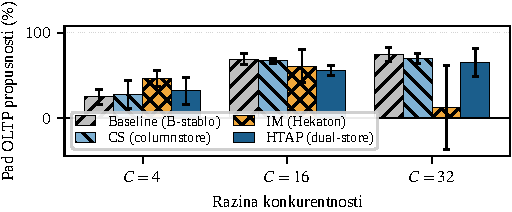
\includegraphics[width=\columnwidth]{figures/fig3_degradation_bs.pdf}
\caption{Pad OLTP propusnosti pri prelasku s omjera 80/20 na 50/50, po
konfiguraciji i razini konkurentnosti (srednja vrijednost $\pm$ standardna
devijacija).}
\label{fig:degradation}
\end{figure}

\subsection{Interferencija pri mješovitom opterećenju}
Pri $C = 16$ prelazak s omjera 80/20 na 50/50 košta CS
67,4\,\%\,$\pm$\,2,8\,\% transakcijske propusnosti, naspram
55,9\,\%\,$\pm$\,6,3\,\% za hibridnu konfiguraciju; razlika od 11,5
procentnih poena statistički je značajna uz veliki efekt
($p < 0{,}001$, $d = 2{,}32$). Slika~\ref{fig:degradation} pokazuje da je ta
prednost ovisna o konkurentnosti: pri $C = 4$ sve konfiguracije gube između
25\,\% i 46\,\% bez značajne razlike CS--HTAP, a pri $C = 32$ usporedbom
dominira varijansa IM konfiguracije, čija je propusnost pri 80/20 i sama
snižena row-mode analitičkim skeniranjima. Mehanizam izolacije je jasan: u CS
batch-mode skeniranja dijele buffer pool i procesorske niti s OLTP naredbama
nad istom disk-zasnovanom shemom, dok u dual-store rasporedu analitički
upiti čitaju \texttt{cs} columnstore, a transakcije rade nad
memorijsko-optimiziranim tabelama koje buffer pool ne dodiruju.
Gubitak 67,4\,\% transakcijskog kapaciteta kritičan je uz ugovorenu razinu
usluge, a red veličine odgovara rasponu od 50 do 70\,\% koji se za
disk-zasnovane sisteme navodi u~\cite{wu2025}.

\subsection{Regresijska analiza}
Dva OLS modela s logaritamski transformisanim zavisnim varijablama
kvantifikuju doprinos svakog faktora (Tabela~\ref{tab:ols}), pri čemu su
Baseline i omjer 80/20 referentne kategorije. Koeficijent HTAP-a od
$+1{,}965$ odgovara $e^{1{,}965} \approx 7{,}1\times$ većoj transakcijskoj
propusnosti od Baseline, dok $-1{,}382$ u modelu latencije odgovara
smanjenju analitičke latencije za $e^{1{,}382} \approx 4{,}0\times$.
Koeficijent CS u modelu propusnosti nije značajan ($p = 0{,}600$): samo
dodavanje columnstore indeksa ne poboljšava transakcijsku propusnost.

\begin{table}[t]
\caption{Koeficijenti OLS regresije ($N = 1\,065$)}
\label{tab:ols}
\centering
\footnotesize
\begin{tabular}{@{}lrrrr@{}}
\toprule
& \multicolumn{2}{c}{$\log(\text{OLTP prop.})$} & \multicolumn{2}{c}{$\log(\text{OLAP } P_{50})$}\\
\cmidrule(lr){2-3}\cmidrule(l){4-5}
\textbf{Parametar} & Koef. & $p$ & Koef. & $p$\\
\midrule
CS naspram Baseline        & $+0{,}021$ & 0,600  & $-0{,}636$ & $<0{,}001$\\
IM naspram Baseline        & $+0{,}708$ & $<0{,}001$ & $-1{,}166$ & $<0{,}001$\\
HTAP naspram Baseline      & $+1{,}965$ & $<0{,}001$ & $-1{,}382$ & $<0{,}001$\\
Omjer 50/50 : 80/20        & $-0{,}821$ & $<0{,}001$ & $+0{,}403$ & $<0{,}001$\\
Omjer 20/80 : 80/20        & $-2{,}211$ & $<0{,}001$ & $+0{,}640$ & $<0{,}001$\\
$\log(\text{konkurentnost})$ & $+0{,}325$ & $<0{,}001$ & $+0{,}395$ & $<0{,}001$\\
\midrule
$R^2$ & \multicolumn{2}{c}{0,881} & \multicolumn{2}{c}{0,854}\\
\bottomrule
\end{tabular}
\end{table}

% =====================================================================
\section{Diskusija}
% =====================================================================
Mjerenja otkrivaju mehanizam koji dosad nije nezavisno kvantifikovan:
columnstore sloj ne samo da ubrzava analitičke upite, nego i \emph{posredno
štiti transakcijske resurse}. Zato dual-store konfiguracija nadmašuje i disk-zasnovane konfiguracije i IM,
koja radi na istom Hekaton engineu. U IM
konfiguraciji analitički upiti skeniraju memorijsko-optimizirane tabele u
row-modu, trošeći znatno više procesorskih ciklusa po redu i zasićujući
procesor pri $C = 16$ i $C = 32$; u dual-store rasporedu opslužuju se
u batch-modu iz columnstore kopije, pa se transakcije nikada ne
natječu s analitičkim nitima za procesor. Ubrzanje analitike je stoga i
sredstvo zaštite OLTP propusnosti --- poluga koja dopunjuje pristup
usmjeren na izolaciju iz~\cite{zhao2023} i razdvojene arhitekture
iz~\cite{huang2020, yang2020}, ovdje ostvarena bez mrežne latencije.

Praktično pravilo je jednostavno: kad god opterećenje spaja transakcije i
analitiku, a preduslovi su ispunjeni, dual-store raspored je poželjniji bez
obzira na omjer; CS ostaje pragmatičan izbor za isključivo analitička
opterećenja, servere s ograničenom memorijom i izdanja
koja ne podržavaju In-Memory OLTP. Preduslovi nisu mali: otprilike
dvostruka potrošnja memorije, trošak održavanja sinhronizacije između
slojeva i tolerancija na analitiku nad podacima koji nisu svježi.

\subsection{Ograničenja validnosti}
\label{sec:threats}
Četiri ograničenja omeđuju ove rezultate. Prvo i najvažnije, ispitana
dual-store konfiguracija razdvaja dva sloja, ali ne izvršava
nikakav mehanizam sinhronizacije (change data capture, replikacija ili
kompakcija), dok produkcijski sistemi tu cijenu plaćaju
kontinuirano~\cite{huang2020, yang2020}; prikazani dobici stoga predstavljaju
gornju granicu ostvarivu uz nultu cijenu sinhronizacije i kvantifikuju
koliko interferencije uklanja fizička separacija, a ne neto dobit potpuno
konzistentnog sistema. Drugo, memorijsko-optimizirane konfiguracije koriste
\texttt{DURABILITY = SCHEMA\_ONLY} i čitaju iz radne memorije, dok
disk-zasnovane čitaju s NVMe SSD-a, pa usporedbe preko različitih medija i
razina trajnosti miješaju efekt arhitekture s efektom medija; najčistije su
usporedbe unutar istog medija (HTAP naspram IM, CS naspram analitičkog sloja
HTAP-a). Treće, asimetrija u \texttt{MAXDOP} postavci koju
zahtijevaju engine-i predstavlja confounding varijablu u usporedbi HTAP--IM,
a njen doprinos nije izolovan. Četvrto, objašnjenje putem zasićenja procesora
izvedeno je iz modela izvršavanja upita, a ne iz direktnog profilisanja, a sva
mjerenja potiču s jedne instance i jednog skupa podataka, pa generalizacija
zahtijeva opreznost.

% =====================================================================
\section{Zaključak}
% =====================================================================
Kroz 1\,070 valjanih serija nad stvarnim skupom od 19,2 miliona zapisa,
dual-store konfiguracija SQL Servera 2022 dominirala je u svakom ispitanom
scenariju mješovitog opterećenja, dostigavši 21\,920 op/s pri $C = 32$ ---
4,6$\times$ više od memorijsko-optimizirane i 9,0$\times$ više od Baseline
konfiguracije --- uz najnižu analitičku latenciju ($P_{50} = 924$\,ms pri
80/20). Čisto memorijsko-optimizirana konfiguracija pokazala se neočekivano
slabom pod mješovitim opterećenjem uprkos istom transakcijskom engineu, jer
row-mode skeniranja zasićuju procesor; disk-zasnovana columnstore
konfiguracija izgubila je dvije trećine kapaciteta čim je dodana analitika. Glavni uvid jeste da je ubrzanje analitike samo po sebi
sredstvo zaštite transakcijske propusnosti; taj posredni efekt, vrijedan
faktora 3,3--6,9, zaslužuje pažnju pri podešavanju HTAP sistema. Buduća
istraživanja mjerit će cijenu kontinuirane sinhronizacije, dodati direktno
profilisanje procesora i proširiti usporedbu na distribuirane sisteme.

\balance

% =====================================================================
\begin{thebibliography}{99}
% popis literature u IEEEtran-ovoj propisanoj veličini od 8 pt (bez izmjene)
\bibitem{diaconu2013}
C. Diaconu \emph{et al.}, ``Hekaton: SQL Server's memory-optimized OLTP
engine,'' in \emph{Proc. ACM SIGMOD}, 2013, pp. 1243--1254.

\bibitem{larson2013}
P.-{\AA}. Larson \emph{et al.}, ``Enhancements to SQL Server column stores,''
in \emph{Proc. ACM SIGMOD}, 2013, pp. 1159--1170.

\bibitem{ozcan2017}
F. \"Ozcan, Y. Tian, and P. T\"oz\"un, ``Hybrid transactional/analytical
processing: A survey,'' in \emph{Proc. ACM SIGMOD}, 2017, pp. 1771--1775.

\bibitem{huang2020}
D. Huang \emph{et al.}, ``TiDB: A Raft-based HTAP database,'' \emph{Proc.
VLDB Endow.}, vol. 13, no. 12, pp. 3072--3084, 2020.

\bibitem{yang2020}
J. Yang \emph{et al.}, ``F1 Lightning: HTAP as a service,'' \emph{Proc. VLDB
Endow.}, vol. 13, no. 12, pp. 3313--3326, 2020.

\bibitem{zhang2024hybench}
C. Zhang, G. Li, and T. Lv, ``HyBench: A new benchmark for HTAP databases,''
\emph{Proc. VLDB Endow.}, vol. 17, no. 5, pp. 939--951, 2024.

\bibitem{zhang2024survey}
C. Zhang, J. Zhou, H. Chen, Z. Wang, and T. Li, ``HTAP databases: A survey,''
\emph{IEEE Trans. Knowl. Data Eng.}, 2024.

\bibitem{song2024}
H. Song, Z. Zhao, X. Ding, and R. Chen, ``A survey on hybrid transactional
and analytical processing,'' \emph{VLDB J.}, 2024.

\bibitem{farber2012}
F. F\"arber, S. K. Cha, J. Primsch, C. Bornh\"ovd, S. Sigg, and W. Lehner,
``SAP HANA database: Data management for modern business applications,''
\emph{ACM SIGMOD Rec.}, vol. 40, no. 4, pp. 45--51, 2012.

\bibitem{lahiri2015}
T. Lahiri \emph{et al.}, ``Oracle Database In-Memory: A dual format in-memory
database,'' in \emph{Proc. IEEE 31st Int. Conf. Data Eng. (ICDE)}, 2015, pp.
1253--1258.

\bibitem{zeng2023}
X. Zeng, M. Abebe, J. Waudby, and A. Pavlo, ``An empirical evaluation of
columnar storage formats,'' \emph{Proc. VLDB Endow.}, vol. 17, no. 2, pp.
148--161, 2023.

\bibitem{larson2015}
P.-{\AA}. Larson \emph{et al.}, ``Real-time analytical processing with SQL
Server,'' \emph{Proc. VLDB Endow.}, vol. 8, no. 12, pp. 1740--1751, 2015.

\bibitem{wu2025}
Y. Wu \emph{et al.}, ``HTAP benchmark in financial scenarios,''
\emph{Security and Safety}, vol. 4, 2025.

\bibitem{zhao2023}
Y. Zhao, J. Chen, Y. Wang, and X. Shi, ``Benchmarking HTAP databases for
performance isolation and real-time analytics,'' \emph{Inf. Syst.}, 2023.

\bibitem{zhao2025pushtap}
P. Zhao \emph{et al.}, ``PUSHtap: PIM-based in-memory HTAP with unified data
storage format,'' in \emph{Proc. 30th ACM ASPLOS}, 2025.

\bibitem{zhang2025synchro}
Y. Zhang \emph{et al.}, ``SynchroStore: A cost-based fine-grained incremental
compaction for hybrid workloads,'' arXiv:2503.18688, 2025.

\bibitem{zhan2025}
C. Zhan \emph{et al.}, ``veDB-HTAP: A highly integrated, efficient and
adaptive HTAP system,'' \emph{Proc. VLDB Endow.}, 2025.
\end{thebibliography}

\end{document}
